\documentclass{cmc}

\begin{document}

\pagestyle{fancy}
\lhead{\textit{\textbf{Computational Motor Control, Spring 2025} \\
    Python exercise, Lab 2, NOT GRADED}} \rhead{Student \\ Names}

\section*{Student names: \ldots (please update)}

\textit{Instructions: Update this file (or recreate a similar one, e.g.\ in
  Word) to prepare your answers to the questions. Feel free to add text,
  equations and figures as needed. Hand-written notes, e.g.\ for the development
  of equations, can also be included e.g.\ as pictures (from your cell phone or
  from a scanner).  \textbf{This lab is not graded. However, the lab exercises
    are meant as a way to familiarise with dynamical systems and to study them
    using Python to prepare you for the final project.} This file does not need
  to be submitted and is provided for your own benefit. The graded exercises
  will have a similar format.}

\textit{The file \fileref{lab\#.py} is provided to run all exercises in
  Python. Each \fileref{exercise\#.py} can be run to run an exercise
  individually. The list of exercises and their dependencies are shown in
  Figure~\ref{fig:files}. When a file is run, message logs will be printed to
  indicate information such as what is currently being run and and what is left
  to be implemented. All warning messages are only present to guide you in the
  implementation, and can be deleted whenever the corresponding code has been
  implemented correctly.}

\begin{figure}[ht]
  \centering 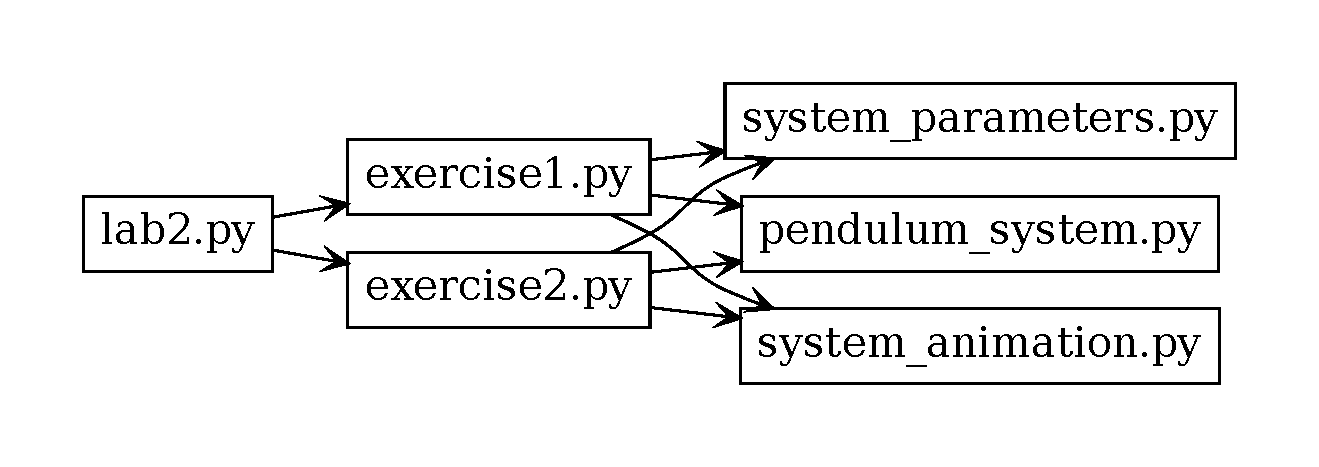
\includegraphics[width=0.5\textwidth]{figures/files}
  \caption{\label{fig:files} Exercise files dependencies. In this lab, you will
    be modifying \fileref{exercise1.py}, \fileref{exercise2.py} and \fileref{pendulum\_system.py}.
    }
\end{figure}

\textit{In this exercise, you will explore the different modeling
  techniques that can be used to control a single joint and
  segment. We initially start by exploring a single joint controlled
  by a a single simplified pendulum model with damping(friction) (exercise1)
  and then extend it to pair of spring-dampers muscle models (exercise2).
  These only represent the passive dynamics observed in a real musculoskeletal system.
  You are provided with a code that can simulate a pair spring-damp muscle model
  . }

\textbf{Important note:}
\textit{Both exercise use a generic class that can handle both a pair of
		spring damp muscles, or a single spring damp muscle sketched in Figure
		\ref{fig:spring_mass_damper_sketch}. Each muscle pair
		contains sping constants and resting angles, and damping coefficients.
		Simply set all the values of these parameters equal for the two pairs
		to study the behavior of a single spring-damper instead of a pair (in Exercise 1).
		Have a look at the specification of parameters of the pendulum
		system in the class \textit{PendulumParameters} in \fileref{system\_parameters.py}.}


\begin{figure}[ht]
  \centering 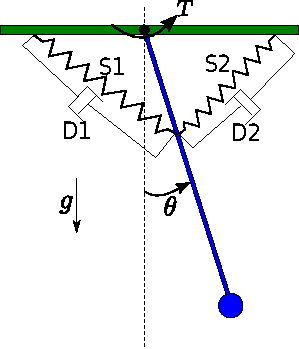
\includegraphics[width=0.2\textwidth]{figures/pendulum_spring_damper}
  \caption[pendulum with spring]{Pendulum model with two springs S1
    and S2 and two dampers b1 and b2\\
    $T$ - Positive torque direction.\\
    $g$ - Gravity.\\
    $\theta$ - Angle made by the pendulum
    \label{fig:spring_mass_damper_sketch} }
\end{figure}


 % ===== exercise 1 ======

\section*{Question 1: Pendulum with friction}

\subsection*{1.a Find the fixed points of the pendulum with friction
  (i.e. damping, and analyze their stability using a local linearization
  under no external input $T_{ext}=0$ ) expressed in the following equation
  (briefly describe the calculation steps). }


\begin{equation}
  \label{eq:ode-pendulum}
  I\ddot{\theta} = -mgLsin(\theta) + T_{ext} - b \dot{\theta}
\end{equation}

Considering Inertia $I = mL^2$, the equation of the pendulum can be
written as,

\begin{equation}
  \label{eq:pendulum}
  \ddot{\theta} = -g\frac{sin(\theta)}{L} + \frac{T_{ext}}{I} - b \frac{\dot{\theta}}{I}
\end{equation}

where $\theta$ is the angle, $g$ the gravity constant, $L$ the length of the pendulum
and $b$ is the damping coefficient.


\corr{\textbf{Fixed points:}}

\corr{
  \begin{equation}
    \label{eq:fixed_points}
    \begin{aligned}
      & \dot{x}_2 = - {g \over L} \sin x_1 - b x_2 & \qquad & sin(\widetilde{x}_1)=0
      \quad \Rightarrow \quad \widetilde{x}_1 = n\pi, \quad n \in Z
      \\
      & \dot{x}_1 = x_2 = 0 & \qquad & \widetilde{x}_2 = 0
    \end{aligned}
  \end{equation}
}

\corr{\textbf{Jacobian and eigenvalues:}}

\corr{
  \begin{equation}
    \label{eq:jacobian}
    J =
    \begin{pmatrix}
      0 & 1 \\ - {g \over L} \cos x_1 & - b
    \end{pmatrix}
    \quad
    \Rightarrow
    \quad
    \lambda^2 + b\lambda + {g \over L} \cos x_1 = 0
    \quad
    \Rightarrow
    \quad
    \lambda_\pm = {-b \pm \sqrt{b^2 - 4{g \over L}\cos x_1} \over 2}
  \end{equation}
}

\corr{In the case where $ \widetilde{x}_1 = 0 $ (i.e. pendulum down), both
  eigenvalues $ \lambda_\pm < 0 $, thus the fixed point is stable. In the case
  $ \widetilde{x}_1 = \pi $, we have $ \lambda_- < 0 $ and $ \lambda_+ > 0 $, thus the fixed
  point is unstable (saddle point).}


\subsection*{1.b Implement the the damping equation of the pendulum using equations described above in the function
  \fileref{pendulum\_system.py::pendulum\_equation}. Numerically solve the differential equations of the pendulum
  with different initial conditions.  Show several time evolutions and phase
  portraits with different initial conditions that illustrate several aspects of
  the interesting behavior of the pendulum. Additionally, implement the damping parameter and demonstrate examples of underdampded, critically damped and overdamped behaviors.
  See \fileref{exercise1.py} and \fileref{system\_parameters.py} and
  \fileref{pendulum\_system.py} for help with implementation.}


\corr{Different time evolutions should be shown. Ideally examples should
  include: starting and staying at unstable fixed point, simple damped
  oscillations around stable fixed point, complete loops due to initial high
  velocity that then end up at stable fixed point. Depending on the choice of
  the parameters, oscillations might disappear in favour of an exponential decay.}

\corr{For instance:}

\begin{figure}[H]
  \centering
  \begin{subfigure}[b]{0.49\textwidth}
    { \centering
      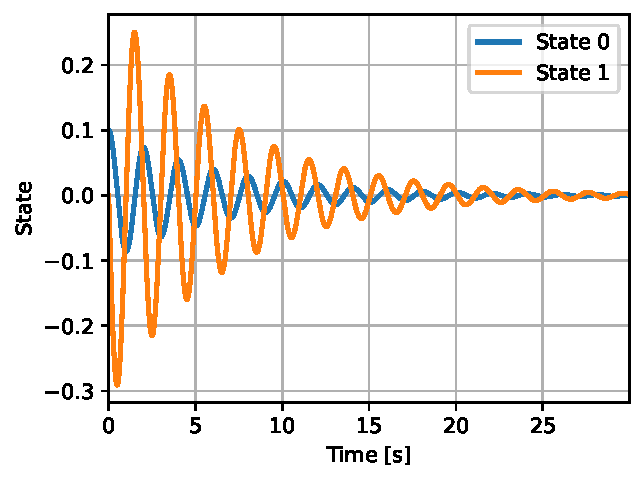
\includegraphics[width=\textwidth]{figures/Normal_case_state_(x0=[0dot1,_0])}
      \label{fig:pendulum-basic-state}
    }
    \caption{\corr{Time evolution}}
  \end{subfigure}
  \begin{subfigure}[b]{0.49\textwidth}
    { \centering
      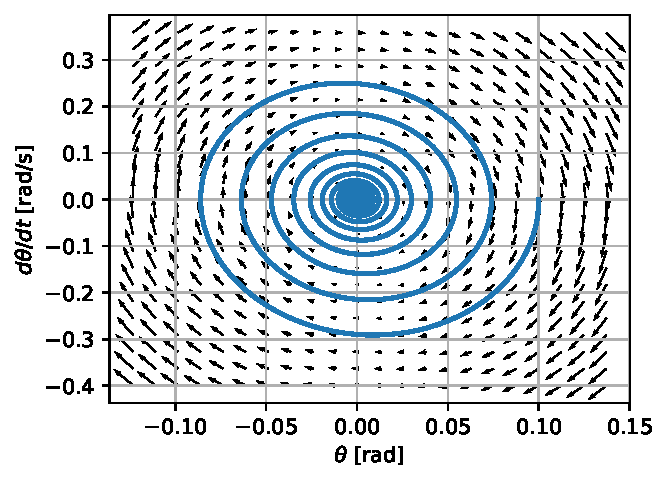
\includegraphics[width=\textwidth]{figures/Normal_case_phase_(x0=[0dot1,_0])}
      \label{fig:pendulum-basic-phase}
    }
    \caption{\corr{Phase portrait}}
  \end{subfigure}
  \caption{\corr{Basic pendulum setup ($ \theta_0 = 0.1~[rad]$, $ \dot{\theta}_0 = 0~[rad/s]$)}}
  \label{fig:pendulum-basic}
\end{figure}

\begin{figure}[H]
  \centering
  \begin{subfigure}[b]{0.49\textwidth}
    { \centering
      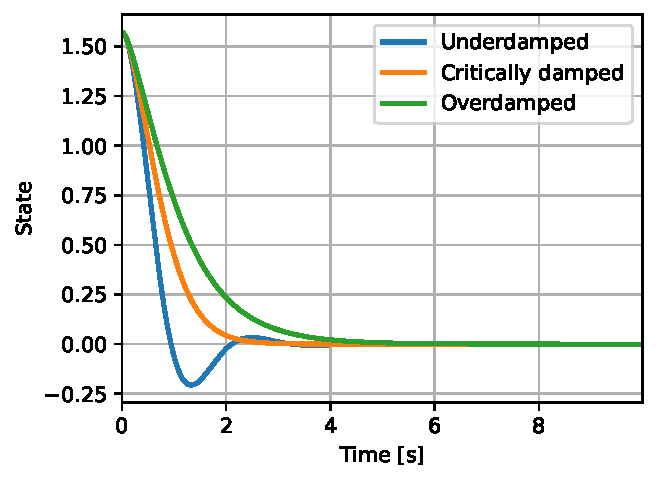
\includegraphics[width=\textwidth]{figures/Fixed_point_types_Temporal_evolution.pdf}
      \label{fig:fixed-point-type-temporal}
    }
    \caption{\corr{Time evolution}}
  \end{subfigure}
  \begin{subfigure}[b]{0.49\textwidth}
    { \centering
      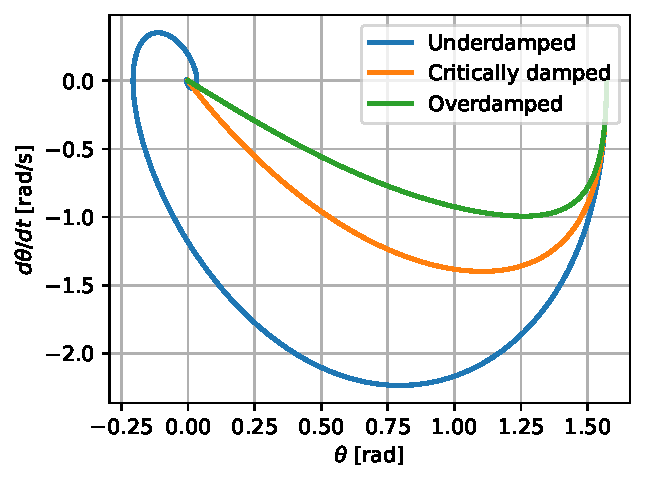
\includegraphics[width=\textwidth]{figures/Fixed_point_types_Phase_plot.pdf}
      \label{fig:fixed-point-type-phase}
    }
    \caption{\corr{Phase portrait}}
  \end{subfigure}
  \caption{\corr{Different types of fixed point are obtained depending on the sign of $ \Delta = b^2 - 4{g \over L}$.
  Note that the underdamped solution shows an overshoot before settling at the equilibrium point.
  Also note that the critically damped solution decays faster than the overdamped (and underdamped) one.} }
  \label{fig:fixed-point-type}
\end{figure}

\begin{figure}[H]
  \centering
  \begin{subfigure}[b]{0.49\textwidth}
    { \centering
      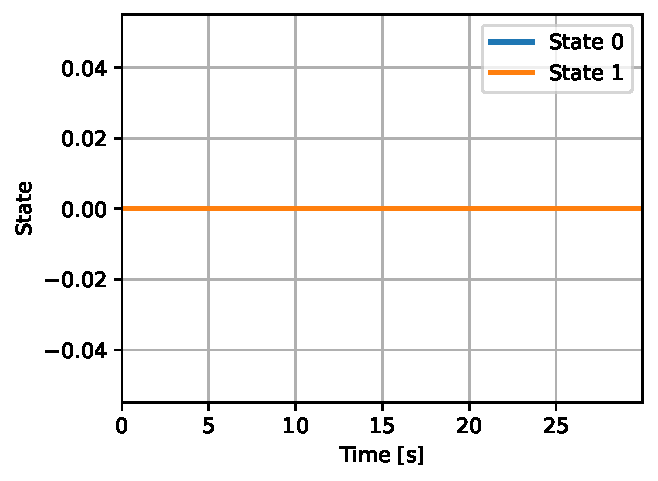
\includegraphics[width=\textwidth]{figures/Stable_case_state_(x0=[0dot0,_0dot0])}
      \label{fig:pendulum-stable-state}
    }
    \caption{\corr{Time evolution}}
  \end{subfigure}
  \begin{subfigure}[b]{0.49\textwidth}
    { \centering
      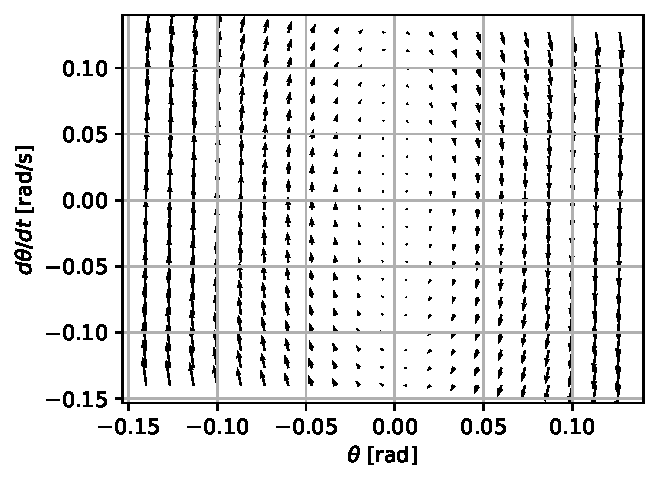
\includegraphics[width=\textwidth]{figures/Stable_case_phase_(x0=[0dot0,_0dot0])}
      \label{fig:pendulum-stable-phase}
    }
    \caption{\corr{Phase portrait}}
  \end{subfigure}
  \caption{\corr{Stable pendulum setup ($ \theta_0 = 0~[rad]$,
      $ \dot{\theta}_0 = 0~[rad/s]$)}}
  \label{fig:pendulum-stable}
\end{figure}

\begin{figure}[H]
  \centering
  \begin{subfigure}[b]{0.49\textwidth}
    { \centering
      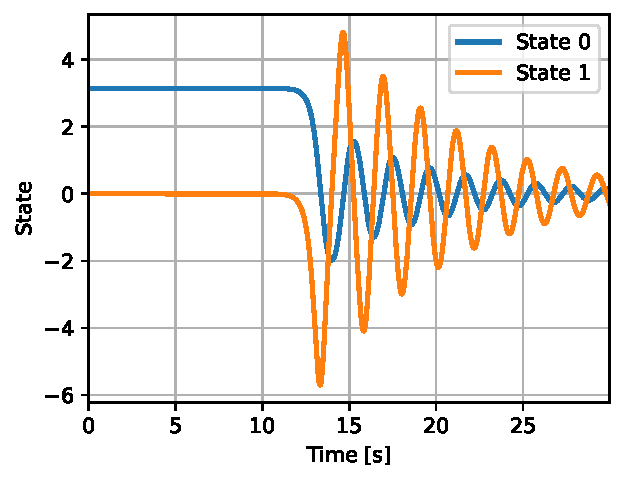
\includegraphics[width=\textwidth]{figures/Unstable_case_state_(x0=[3dot141592653589793,_0dot0])}
      \label{fig:pendulum-unstable-state}
    }
    \caption{\corr{Time evolution}}
  \end{subfigure}
  \begin{subfigure}[b]{0.49\textwidth}
    { \centering
      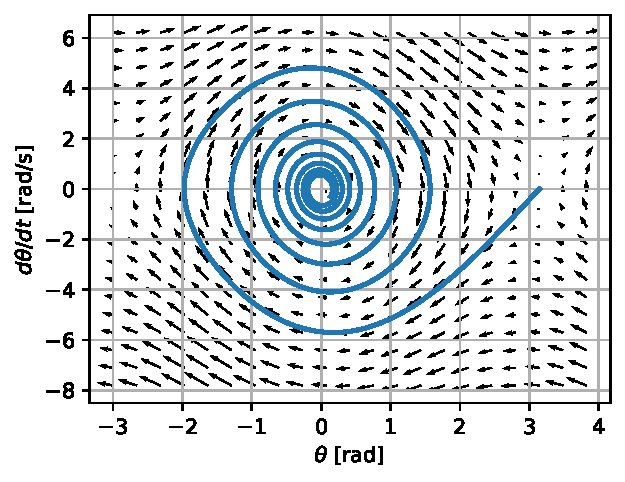
\includegraphics[width=\textwidth]{figures/Unstable_case_phase_(x0=[3dot141592653589793,_0dot0])}
      \label{fig:pendulum-unstable-phase}
    }
    \caption{\corr{Phase portrait}}
  \end{subfigure}
  \caption{\corr{Unstable pendulum setup ($ \theta_0 = \pi~[rad] $,
      $ \dot{\theta}_0 = 0~[rad/s] $). The pendulum stays at the unstable fixed point
      for a few seconds, and then is pushed away due to numerical imprecision of
      the integration. It ends up at the stable fixed point (0,0)}}
  \label{fig:pendulum-unstable}
\end{figure}

\begin{figure}[H]
  \centering
  \begin{subfigure}[b]{0.49\textwidth}
    { \centering
      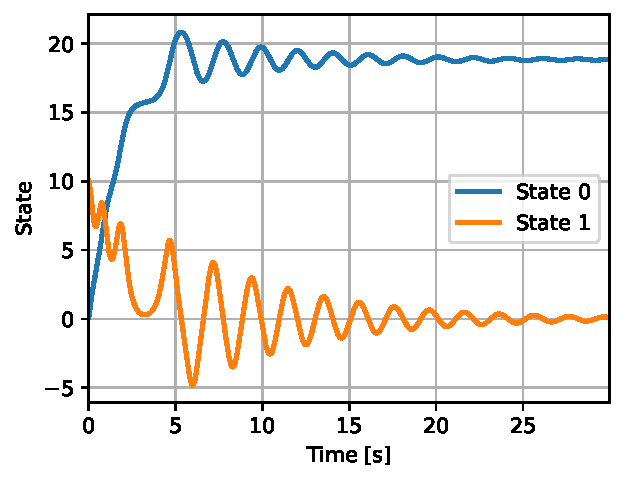
\includegraphics[width=\textwidth]{figures/Multiple_loops_case_state_(x0=[0dot1,_10dot0])}
      \label{fig:pendulum-high-vel-state}
    }
    \caption{\corr{Time evolution}}
  \end{subfigure}
  \begin{subfigure}[b]{0.49\textwidth}
    { \centering
      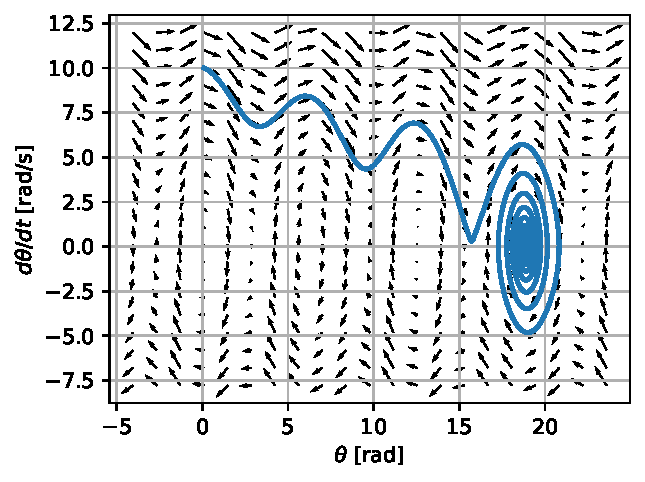
\includegraphics[width=\textwidth]{figures/Multiple_loops_case_phase_(x0=[0dot1,_10dot0])}
      \label{fig:pendulum-high-vel-phase}
    }
    \caption{\corr{Phase portrait}}
  \end{subfigure}
  \caption{\corr{High initial velocity pendulum setup ($ \theta_0 = 0.1~[rad] $,
      $ \dot{\theta}_0 = 10~[rad/s] $). In this case, the pendulum has a high initial
      velocity, and therefore makes three complete rotations before converging
      to the stable fixed point (6 pi, 0).}}
  \label{fig:pendulum-high-vel}
\end{figure}


\subsection*{1.c Investigate and describe how the behavior of the pendulum
  changes if friction is zero (b=0).  Show a new phase portrait.}


\begin{figure}[H]
  \centering
  \begin{subfigure}[b]{0.49\textwidth}
    { \centering
      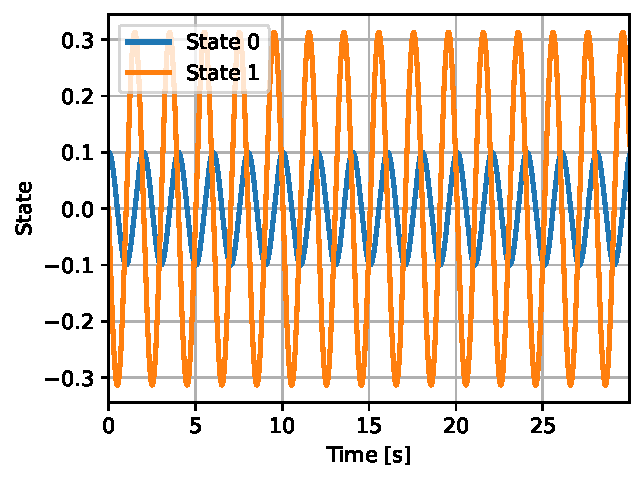
\includegraphics[width=\textwidth]{figures/State_without_damping_(x0=[0dot1,_0])}
      \label{fig:pendulum-no-friction-state}
    }
    \caption{\corr{Time evolution}}
  \end{subfigure}
  \begin{subfigure}[b]{0.49\textwidth}
    { \centering
      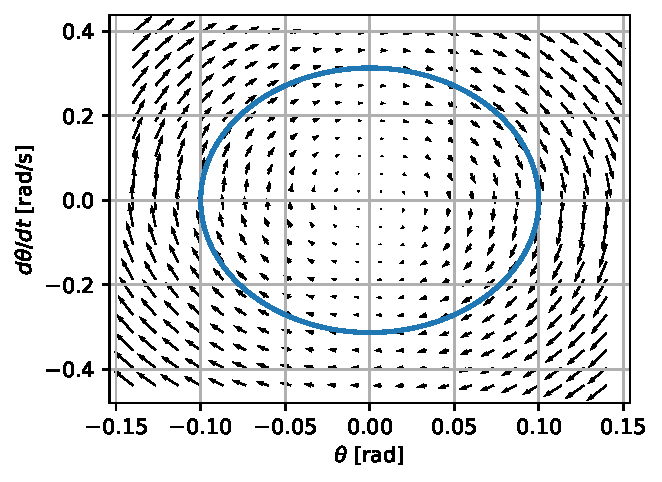
\includegraphics[width=\textwidth]{figures/Phase_without_damping_(x0=[0dot1,_0])}
      \label{fig:pendulum-no-friction-phase}
    }
    \caption{\corr{Phase portrait}}
  \end{subfigure}
  \caption{\corr{Periodic pendulum setup ($ \theta_0 = 0.1~[rad] $,
      $ \dot{\theta}_0 = 0~[rad/s] $). The figures show that without friction the
      pendulum keeps oscillating without reduction of amplitude of
      oscillation. The fixed points, both unstable and stable, have not
      changed.}}
  \label{fig:pendulum-no-friction}
\end{figure}


\subsection*{1.d Does the pendulum without friction (b=0) produce stable limit
  cycles? Discuss, and try to support your statement with some numerical
  simulations (show figures) and/or analytical arguments.}


\begin{figure}[H]
  \centering
  \begin{subfigure}[b]{0.49\textwidth}
    { \centering
      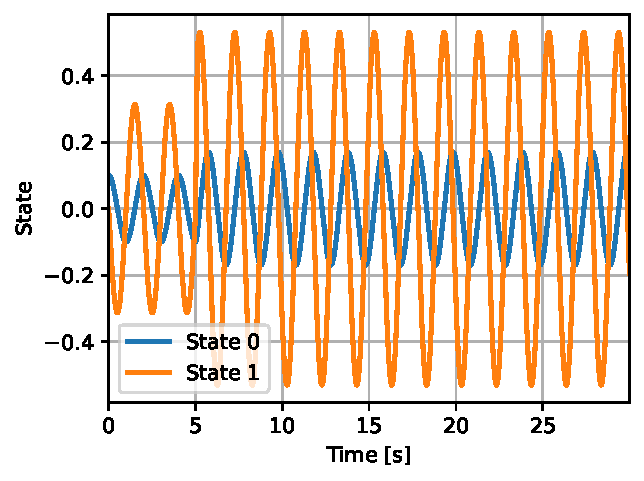
\includegraphics[width=\textwidth]{figures/State_with_perturbation_(x0=[0dot1,_0])}
      \label{fig:pendulum-no-friction-stable-limit-state}
    }
    \caption{\corr{Time evolution}}
  \end{subfigure}
  \begin{subfigure}[b]{0.49\textwidth}
    { \centering
      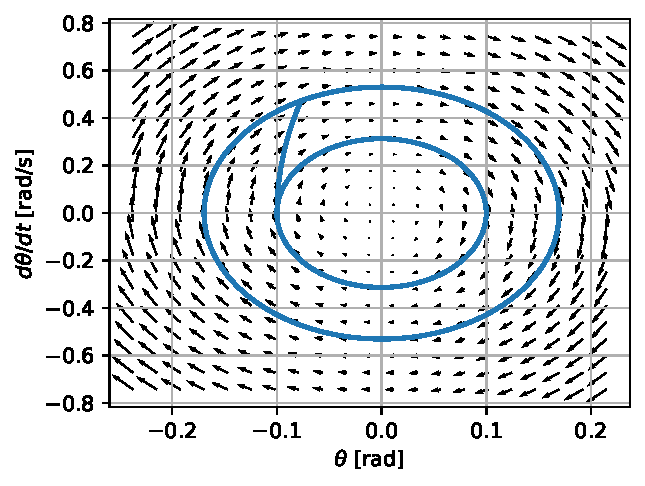
\includegraphics[width=\textwidth]{figures/Phase_with_perturbation_(x0=[0dot1,_0])}
      \label{fig:pendulum-no-friction-stable-limit-phase}
    }
    \caption{\corr{Phase portrait}}
  \end{subfigure}
  \caption{\corr{The pendulum without friction does not produce stable limit
      cycle behavior. It has multiple closed orbits that are not
      isolated. Perturbations lead to new orbits.}}
  \label{fig:pendulum-no-friction-stable-limit}
\end{figure}


\subsection*{1.e Investigate how the behavior of the pendulum changes if the
  viscous friction term is replaced with a dry (Coulomb) friction term. Unlike
  viscous friction, dry friction does not depend on speed, only the direction of
  movement. What are the main differences between the two types of pendulum?
  (discuss and show some examples). And is there anything notable about the
  numerical integration of the pendulum with dry friction? If yes, what and why?}

\begin{equation}
  \label{eq:ode-pendulum-dry}
  \ddot{\theta} = - {g \over L} \sin \theta - b \cdot sign(\dot{\theta})
\end{equation}


\begin{figure}[H]
  \centering
  \begin{subfigure}[b]{0.49\textwidth}
    { \centering
      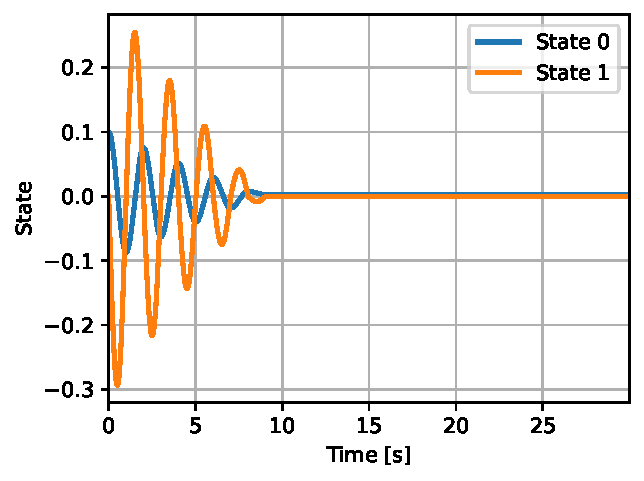
\includegraphics[width=\textwidth]{figures/State_with_dry_friction_(x0=[0dot1,_0])}
      \label{fig:pendulum-basic-state}
    }
    \caption{\corr{Time evolution}}
  \end{subfigure}
  \begin{subfigure}[b]{0.49\textwidth}
    { \centering
      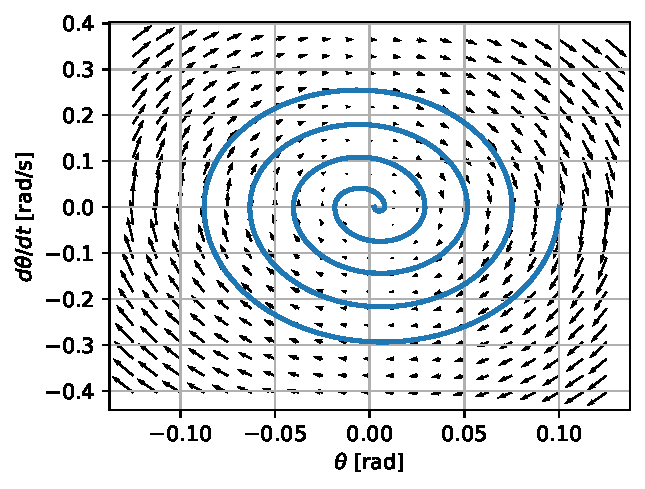
\includegraphics[width=\textwidth]{figures/Phase_with_dry_friction_(x0=[0dot1,_0])}
      \label{fig:pendulum-basic-phase}
    }
    \caption{\corr{Phase portrait}}
  \end{subfigure}
  \caption{\corr{Pendulum with dry friction}}
  \label{fig:pendulum-basic}
\end{figure}

\corr{This represents a stiff dynamical system, i.e. a system that is difficult
  to integrate numerically.  Indeed, this pendulum is difficult to solve
  numerically because of the switch of derivatives when the angular velocity
  changes sign (friction jumping between b and –b). Many more integration times
  steps are needed than for the pendulum with viscous friction. The higher d,
  the more difficulties the integration method has.}

\corr{Fixed points are different from the pendulum with viscous friction. Quite
  complex behavior: the pendulum ends in a position/angle that depends on the
  initial conditions (not anymore with a vertical position).}





 % ===== exercise 2 ======

\section*{Exercise 2 : Pendulum model with passive elements}
\label{sec:question-1}

Mechanical behavior of muscle tissue can be approximated by simple
passive elements such as springs and dampers. These elements, when
combined properly, allow to study the behavior of muscle under
compressive and tensile loads.

Consider the following equation describing the motion of simple
pendulum with an external torque $T_{ext}$,

\begin{equation}
  \label{eq:pendulum_1}
  I\ddot{\theta} = -mgLsin(\theta) + T_{ext}
\end{equation}


Consider the system only for the pendulum range $\theta$ =
$[-\pi/2, \pi/2]$

\subsection*{Explore the pendulum model with two antagonist spring
  elements}

In this question the goal is to add two antagonist springs to the
pendulum model which you are already familiar with from lab 2
exercises. For simplicity we assume the springs directly apply a
torsional force on to the pendulum.  Use equation \ref{eqn:spring} to
develop the spring model.

\textit{\textbf{Note} : The springs can only produce force in
  one-direction like the muscles.  That is, they can only apply a
  pulling force and apply a zero force when compressed.  In terms of
  torsion this translates to, spring S1 can exert only clockwise
  torque and spring S2 can exert only counter-clockwise torque.  You
  need to accommodate for this condition in the equations shown below.}

The setup for the pendulum with a pair of antagonist springs is as
shown in figure \ref{fig:pendulum_spring}. Use \fileref{exercise2.py},
\fileref{pendulum\_system.py} and \fileref{system\_parameters.py} files to
complete the exercise.


\begin{figure}[H]
  \centering
  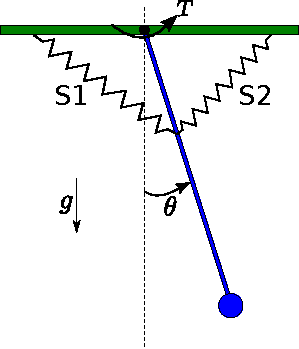
\includegraphics[width=.3\textwidth]{figures/pendulum_spring}
  \caption[pendulum with spring]{Pendulum model with two springs S1
    and S2.\\
    $T$ - Positive torque direction.\\
    $g$ - Gravity.\\
    $\theta$ - Angle made by the pendulum}
  \label{fig:pendulum_spring}
\end{figure}


\begin{equation}
  \label{eqn:spring}
  T_{S} = k \cdot (\theta_{ref} - \theta)
\end{equation}

Where,
\begin{itemize}
\item $T_{S}$ : Torsional Spring force
\item $k$ : Spring Constant
\item $\theta_{ref}$ : Spring reference angle
\item $\theta$ : pendulum angle
\end{itemize}

Substituting the above in \ref{eq:pendulum},

\begin{eqnarray}
  \label{eq:spring}
  \ddot{\theta} = -g\frac{sin(\theta)}{L} + \frac{T_{ext}}{I} + \frac{T_{S}}{I} \\
  \ddot{\theta} = -g\frac{sin(\theta)}{L} + \frac{T_{ext}}{I} + \frac{k \cdot (\theta_{ref} - \theta)}{I} \label{eq:genSpring}
\end{eqnarray}

Use the generalized form of the spring equation described in
\ref{eq:genSpring} to extend it to both the antagonist springs S1 and
S2 with the necessary conditions to make sure springs do not produce
when compressed.

\corr{Extending the above equation to both springs,}

\begin{equation}
  \corr{\ddot{\theta} = -g\frac{sin(\theta)}{L} + min(\frac{k1 \cdot (\theta_{ref1} - \theta)}{I}, 0) + max(\frac{k2 \cdot (\theta_{ref2} - \theta)}{I}, 0)+ \frac{T_{ext}}{I}}
\end{equation}

\corr{For all questions the initial conditions used are,
  $$\theta = 0.5 $$
  $$\dot{\theta} = 0.1$$
  unless explicity specificied otherwise.  Students may use different
  set of initial conditions}

\subsection*{2.a Implement the dynamic equations of the pendulum with
  springs using equations described above in the function
  \fileref{pendulum\_system.py::pendulum\_equation}.  Does the system
  have a stable limit cycle behavior?  Describe and run an experiment
  to support your answer. You can use the function
  \fileref{exercise2.py::pendulum\_perturbation} to perturb the
  pendulum either by changing states or applying an external torque.
  Use the class \fileref{system\_animation.py::SystemAnimation} to
  visualize the pendulum. Example code can be found in
  \fileref{exercise2.py::exercise2}}
\label{subsec:2.a}


\corr{The first requirement for a limit cycle is that the system
  should have a closed trajectory. The pendulum system with springs
  does exhibit a closed trajectory behavior. But, in order to have a
  stable limit cycle the system should converge to a single trajectory
  as time tends to either positive/negative infinity.  One solution to
  check for stable limit cycle behavior is to use the state and phase
  plot like shown in figure \ref{fig:pendulum-spring-limit-cycle}
  under perturbations to show that there is no stable limit cycle
  behavior. At t=5s a pertubation is applied to the velocity of the
  system ($\dot{\theta} = 2.0$). This pushes the trajectory to a new
  trajectory and it never returns to the original trajectory. This
  shows that the system does not have a stable limit cycle.
  Alternatively students may also use poincare map to show that there
  is no stable limit cycle. \textit{Students should clearly detail the
    pertubation they used.}}

\begin{figure}[H]
  \centering
  \begin{subfigure}[b]{0.49\textwidth}
    { \centering
      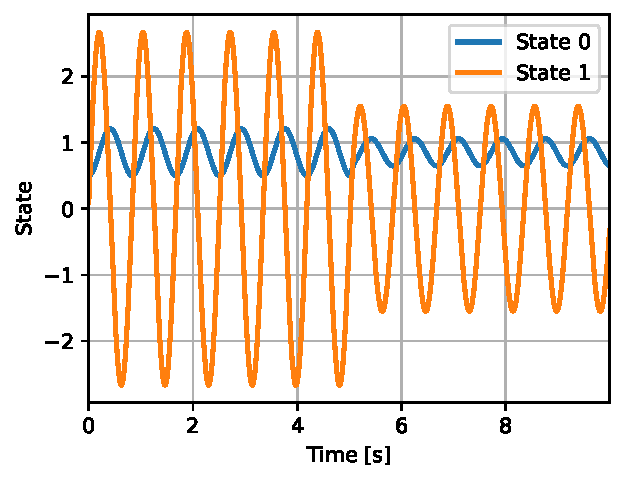
\includegraphics[width=\textwidth]{figures/State_Limit_Cycle(x0_=_[0dot5,_0dot1]).pdf}
      \label{fig:spring_state}
    }
    \caption{State of pendulum with spring under perturbations}
  \end{subfigure}
  \begin{subfigure}[b]{0.49\textwidth}
    { \centering
      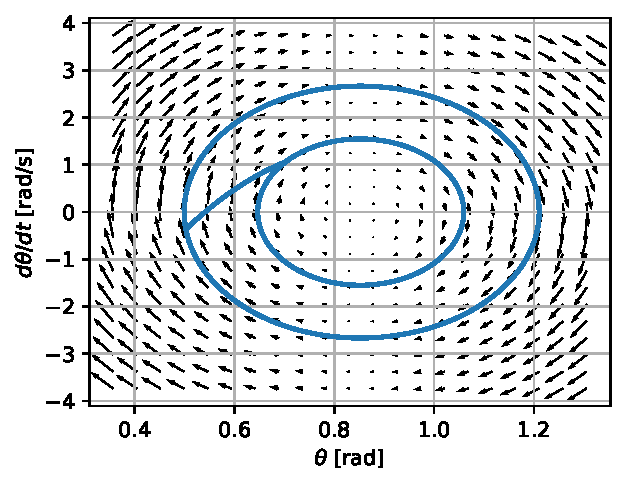
\includegraphics[width=\textwidth]{figures/Phase_Limit_Cycle(x0_=_[0dot5,_0dot1]).pdf}
      \label{fig:spring_phase}
    }
    \caption{Phase of pendulum with spring under perturbations}
  \end{subfigure}
  \caption{\corr{Pertubation approach to check to system limit cycle
      behavior}}
  \label{fig:pendulum-spring-limit-cycle}
\end{figure}

\subsection*{2.b Explore the role of spring constant ($k$) and spring
  reference angle ($\theta_{ref}$) in terms of range of motion,
  amplitude and frequency of pendulum. Keep the constants equal, i.e
  $k_1$  = $k_2$ and $\theta_{ref1} = \theta_{ref2}$
  \\ Refer to \fileref{exercise2.py::exercise1} for an example}


\corr{\textbf{Spring constant (k):} Dictates the magnitude and rate at which
  the pendulum oscillates. The larger the constant the faster the
  system oscillates. This can also be seen as the responsiveness of
  the system. Figure \ref{fig:pendulum-spring-constant-1} shows the
  reponse of the pendulum with a small spring constant of
  $k_1 = k_2 = 0.1$. Figure \ref{fig:pendulum-spring-constant-2} shows
  the reponse of the pendulum with a large spring constant of
  $k_1 = k_2 = 100$.
  \begin{itemize}
  \item For both low/high spring constant, the amplitude of the
    $\theta$ remains the same while the amplitude of $\dot{\theta}$
    increases with increase in spring constant magnitude.
  \item The frequency of both $\theta$ and $\dot{\theta}$ increases
    with higher spring constant and vice-versa.
  \end{itemize}
}

\corr{\textbf{Reference angle:} The resting angle for the spring. Since the
  spring like muscles act only in one direction, the resting angle
  dictates the angular position of the pendulum at which springs start
  to act.  But having a symmetric spring reference angle for both
  springs leads to no change in amplitude, range of motion or
  frequency for a given set of initial conditions. Figures
  \ref{fig:pendulum-spring-reference-1} and
  \ref{fig:pendulum-spring-reference-2} show the state and phase plot
  of the system with spring references close to reference
  ($\theta_{ref1} = -10^\circ $ \& $\theta_{ref1} = 10^\circ $ ) and
  far from reference ($\theta_{ref1} = -75^\circ$ \&
  $\theta_{ref2} = 75^\circ$ ) respectively. With reference being
  $\theta = 0.0^\circ$}

%%%%%%%%%%%%%%% SPRING CONSTANT %%%%%%%%%%%%%%%

\begin{figure}[H]
  \centering
  \begin{subfigure}[b]{0.49\textwidth}
    { \centering
      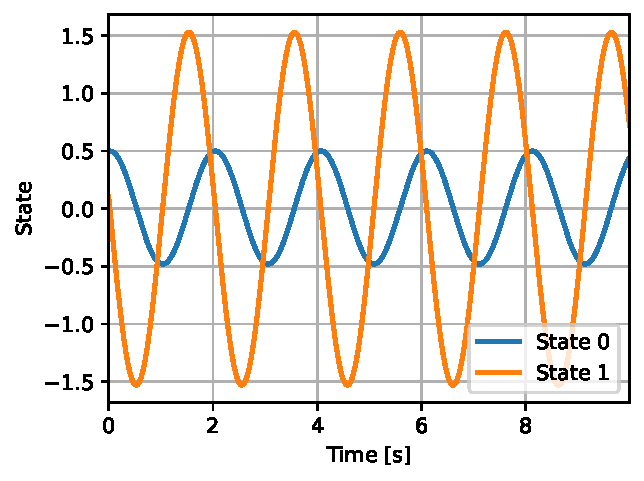
\includegraphics[width=\textwidth]{figures/State_Spring_Constant_1(x0_=_[0dot5,_0dot1]).pdf}
    }
    \caption{State of pendulum with low spring constant}
    \label{fig:state-pendulum-spring-constant-1}
  \end{subfigure}
  \begin{subfigure}[b]{0.49\textwidth}
    { \centering
      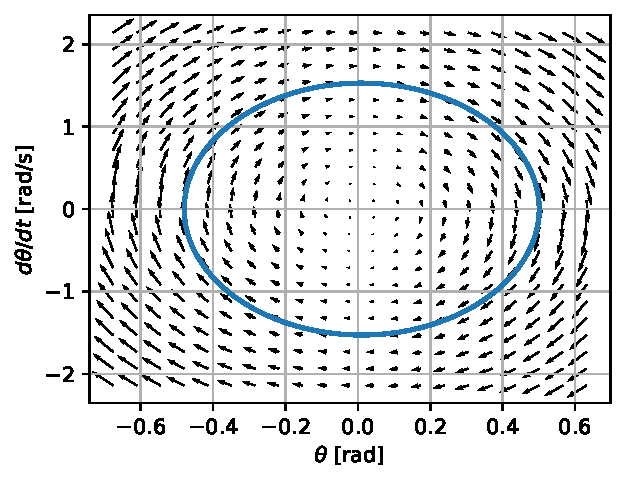
\includegraphics[width=\textwidth]{figures/Phase_Spring_Constant_1(x0_=_[0dot5,_0dot1]).pdf}
    }
    \caption{Phase of pendulum with low spring constant}
    \label{fig:phase-pendulum-spring-constant-1}
  \end{subfigure}
  \caption{\corr{State of pendulum with spring to study the effect of
      spring constant}}
  \label{fig:pendulum-spring-constant-1}
\end{figure}

\begin{figure}[H]
  \centering
  \begin{subfigure}[b]{0.49\textwidth}
    { \centering
      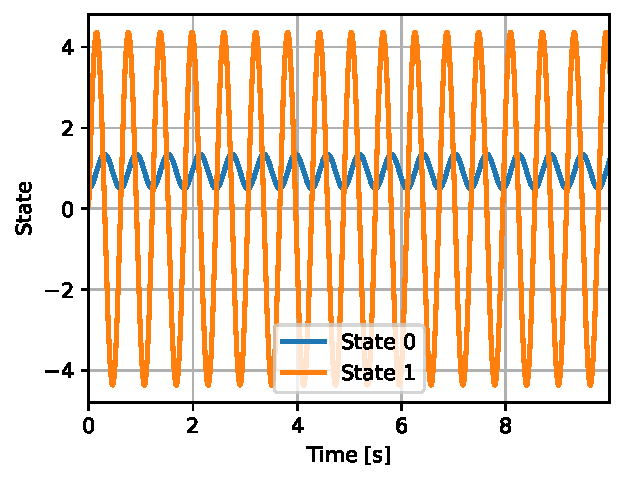
\includegraphics[width=\textwidth]{figures/State_Spring_Constant_2(x0_=_[0dot5,_0dot1]).pdf}
    }
    \caption{State of pendulum with high spring constant}
    \label{fig:state-pendulum-spring-constant-2}
  \end{subfigure}
  \begin{subfigure}[b]{0.49\textwidth}
    { \centering
      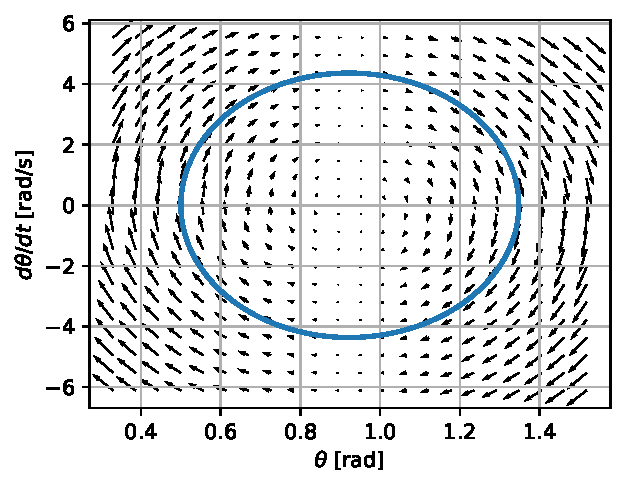
\includegraphics[width=\textwidth]{figures/Phase_Spring_Constant_2(x0_=_[0dot5,_0dot1]).pdf}
    }
    \caption{Phase of pendulum with high spring constant}
    \label{fig:phase-pendulum-spring-constant-2}
  \end{subfigure}
  \caption{\corr{State of pendulum with spring to study the effect of
      spring constant}}
  \label{fig:pendulum-spring-constant-2}
\end{figure}

%%%%%%%%%%%%%%% SPRING REFERENCE %%%%%%%%%%%%%%%

\begin{figure}[H]
  \centering
  \begin{subfigure}[b]{0.49\textwidth}
    {
      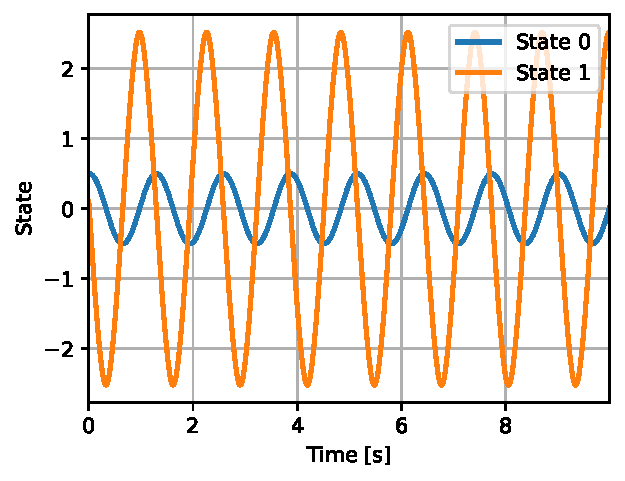
\includegraphics[width=\textwidth]{figures/State_Spring_Reference_1(x0_=_[0dot5,_0dot1]).pdf}
    }
    \caption{State of pendulum with reference close to pendulum rest
      position}
    \label{fig:state-pendulum-spring-reference-1}
  \end{subfigure}
  \begin{subfigure}[b]{0.49\textwidth}
    { \centering
      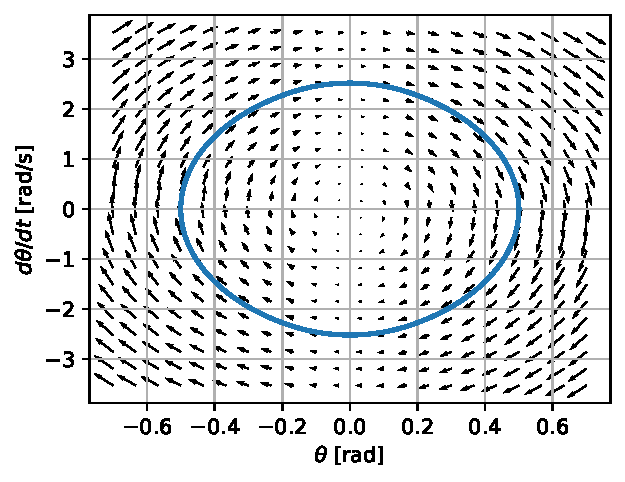
\includegraphics[width=\textwidth]{figures/Phase_Spring_Reference_1(x0_=_[0dot5,_0dot1]).pdf}
    }
    \caption{Phase of pendulum with reference close to pendulum rest
      position}
    \label{fig:phase-pendulum-spring-reference-1}
  \end{subfigure}
  \caption{\corr{State of pendulum with spring to study the effect of
      spring reference}}
  \label{fig:pendulum-spring-reference-1}
\end{figure}


\begin{figure}[H]
  \centering
  \begin{subfigure}[b]{0.49\textwidth}
    { \centering
      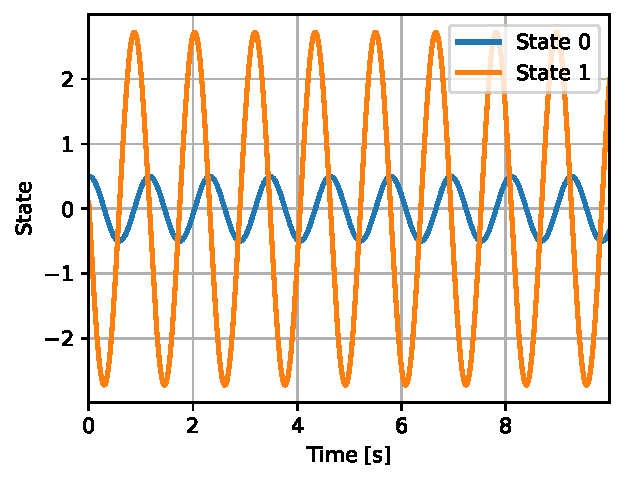
\includegraphics[width=\textwidth]{figures/State_Spring_Reference_2(x0_=_[0dot5,_0dot1]).pdf}
    }
    \label{fig:state-pendulum-spring-reference-2}
    \caption{State of pendulum with reference far to pendulum rest
      position}
  \end{subfigure}
  \begin{subfigure}[b]{0.49\textwidth}
    { \centering
      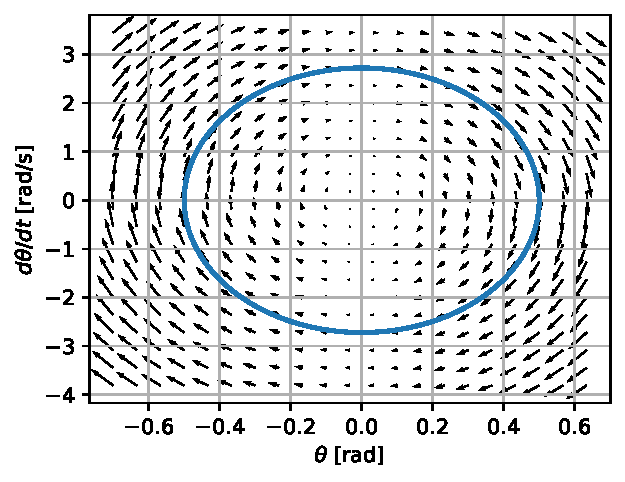
\includegraphics[width=\textwidth]{figures/Phase_Spring_Reference_2(x0_=_[0dot5,_0dot1]).pdf}
    }
    \label{fig:phase-pendulum-spring-reference-2}
    \caption{Phase of pendulum with reference far to pendulum rest
      position}
  \end{subfigure}
  \caption{\corr{State of pendulum with spring to study the effect of
      spring reference}}
  \label{fig:pendulum-spring-reference-2}
\end{figure}


\subsection*{2.c Explain the behavior of the model when you have
  asymmetric spring constants ($k$) and spring reference angles
  ($\theta_{ref}$), i.e. $k_1 \neq k_2$ and $\theta_{ref1} \neq \theta_{ref2}$
  Support your responses with relevant plots}


%%%%%%%%%%%%%%% DIFFERENT SPRING CONSTANT AND REFERENCE
%%%%%%%%%%%%%%% BEHAVIOR %%%%%%%%%%%%%%%

\corr{As we saw the previous question, changing the spring constant
  and reference angle yielded different behaviors. Here we introduce
  assymetry in the system and change parameters individually.}

\corr{\textbf{Variable Spring Constant (k):} In figure
  \ref{fig:pendulum-variable-spring-constant-1} the spring constants
  are set to $k_1 = 1.0$ and $k_2 = 100.$ and both spring references
  set to $\theta_{ref1} = \theta_{ref2} = 0.0 ^\circ$. With these
  values, it is clear from the phase plot
  \ref{fig:phase-pendulum-variable-spring-constant-1} that variable
  spring constants introduces assymetry in the shape of the closed
  trajectory. The side with higher spring constant pulls the pendulum
  back to the reference faster. While the slower spring side is
  dominated more by the pendulum dynamics rather than of the spring
  forces.}

\corr{\textbf{Variable Spring reference ($\theta_{ref}$):} In figure
  \ref{fig:pendulum-variable-spring-reference-1} the spring references
  are set to $\theta_{ref1} = 0.0^\circ$ and
  $\theta_{ref2} = 75.^\circ$ and both spring constants set to
  $k_1 = k_2 = 10.0$. With these values, the it is clear from the
  phase plot \ref{fig:phase-pendulum-variable-spring-reference-1} that
  variable spring references changes the center of the closed
  trajectory. That is, the pendulum system now oscillates around a
  non-zero point.}


\corr{Thus by having unssymetric spring values, we can produce more
  complex closed loop trajectories in a simple system.}

\begin{figure}[H]
  \centering
  \begin{subfigure}[b]{0.49\textwidth}
    { \centering
      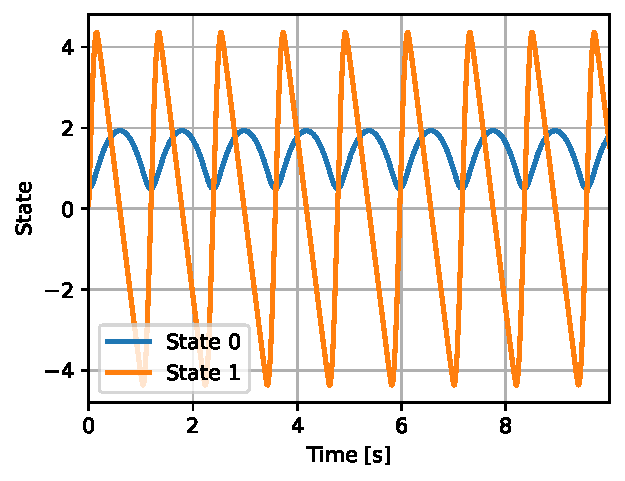
\includegraphics[width=\textwidth]{figures/State_Variable_Spring_Constant_1(x0_=_[0dot5,_0dot1]).pdf}
    }
    \caption{State of pendulum with Variable spring constant}
    \label{fig:state-pendulum-variable-spring-constant-1}
  \end{subfigure}
  \begin{subfigure}[b]{0.49\textwidth}
    { \centering
      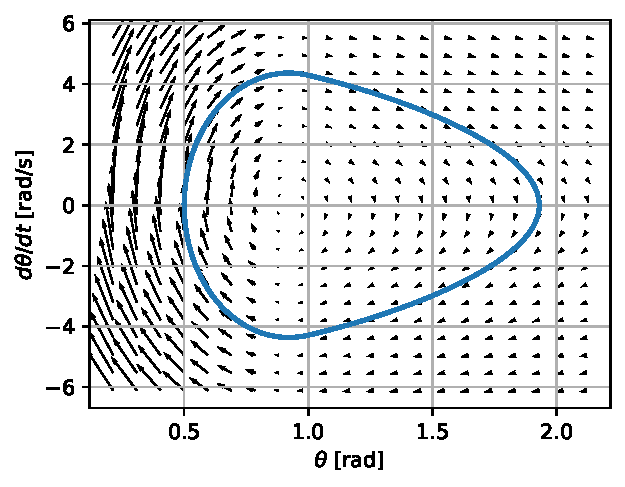
\includegraphics[width=\textwidth]{figures/Phase_Variable_Spring_Constant_1(x0_=_[0dot5,_0dot1]).pdf}
    }
    \caption{Phase of pendulum with Variable spring constant}
    \label{fig:phase-pendulum-variable-spring-constant-1}
  \end{subfigure}
  \caption{\corr{State of pendulum with spring to study the effect of
      Variable spring constant}}
  \label{fig:pendulum-variable-spring-constant-1}
\end{figure}

\begin{figure}[H]
  \centering
  \begin{subfigure}[b]{0.49\textwidth}
    { \centering
      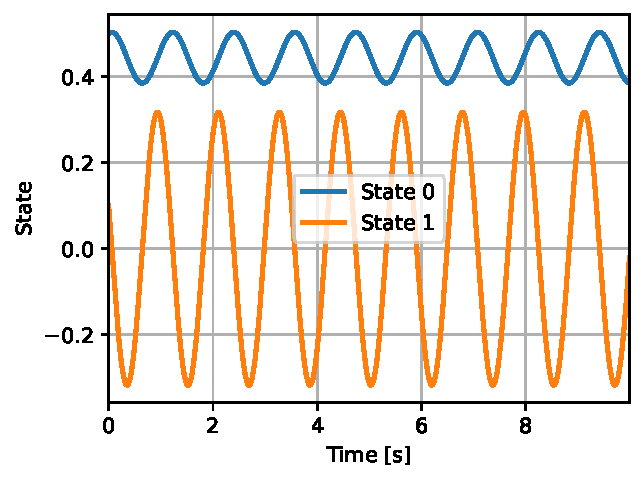
\includegraphics[width=\textwidth]{figures/State_Variable_Spring_Reference_1(x0_=_[0dot5,_0dot1]).pdf}
    }
    \caption{State of pendulum with Variable spring reference}
    \label{fig:state-pendulum-variable-spring-reference-1}
  \end{subfigure}
  \begin{subfigure}[b]{0.49\textwidth}
    { \centering
      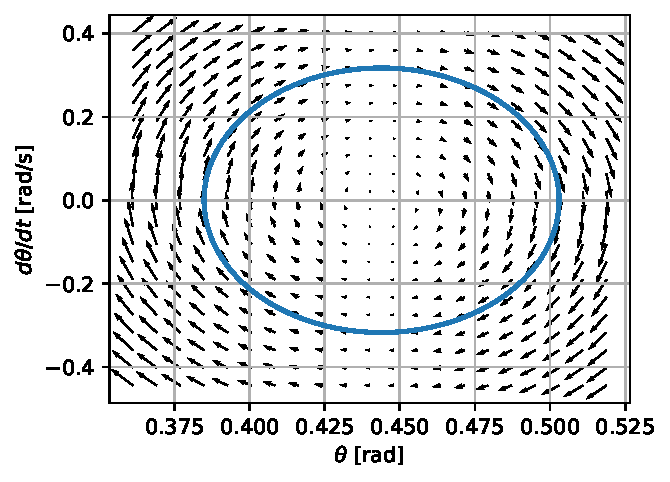
\includegraphics[width=\textwidth]{figures/Phase_Variable_Spring_Reference_1(x0_=_[0dot5,_0dot1]).pdf}
    }
    \caption{Phase of pendulum with Variable spring reference}
    \label{fig:phase-pendulum-variable-spring-reference-1}
  \end{subfigure}
  \caption{\corr{State of pendulum with spring to study the effect of
      variable spring reference}}
  \label{fig:pendulum-variable-spring-reference-1}
\end{figure}

\newpage

\subsection*{Explore the pendulum model with two antagonist spring and damper elements}
Over time muscles lose energy while doing work. In order to account
for this property, let us now add a damper in parallel to the spring
model. Use equation \ref{eqn:damper} to develop the damper model.

\textit{\textbf{Note} : Like the previous springs, the springs in spring-dampers
  can only produce a force in one-direction.  However, the damper terms do not
  have this limitation and each damper can exert a force in both directions.}

Again use \fileref{exercise2.py}, \fileref{pendulum\_system.py} and
\fileref{system\_parameters.py} files to complete the exercise. The
setup for the pendulum model with a pair of antagonist spring and
dampers in parallel is as shown in figure
\ref{fig:pendulum_spring_damper}.


\begin{figure}[H]
  \centering
  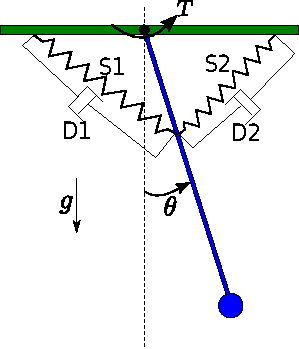
\includegraphics[width=.3\textwidth]{figures/pendulum_spring_damper}
  \caption[pendulum with spring]{Pendulum model with two springs S1
    and S2 and two dampers b1 and b2\\
    $T$ - Positive torque direction.\\
    $g$ - Gravity.\\
    $\theta$ - Angle made by the pendulum}
  \label{fig:pendulum_spring_damper}
\end{figure}



\begin{equation}
  \label{eqn:damper}
  T_{B} = b \cdot \dot{\theta}
\end{equation}

Where,
\begin{itemize}
\item $T_{B}$ : Torsional Damper force
\item $b$ : Damping Constant
\item $\dot{\theta}$ : pendulum angular velocity
\end{itemize}

The combined spring damper torque is given by,
\begin{equation}
  \label{eq:spring_damper}
  T_{S} - T_{B} = k \cdot (\theta_{ref} - \theta) - b \cdot \dot{\theta}
\end{equation}

The minus for the damper comes from the fact that damper is acting
against the work done by the spring.

Substituting the above in \ref{eq:pendulum}

\begin{eqnarray}
  \label{eq:spring-damper}
  \ddot{\theta} = -g\frac{sin(\theta)}{L} + \frac{T_{ext}}{I} + \frac{T_{S} - T_{B}}{I} \\
  \ddot{\theta} = -g\frac{sin(\theta)}{L}+ \frac{T_{ext}}{I} + (\frac{k \cdot (\theta_{ref} - \theta) - b \cdot \dot{\theta}}{I}) \label{eq:genSpringDamper}
\end{eqnarray}

Use the generalized form of the spring equation described in
\ref{eq:genSpringDamper} to extend it to both the antagonist
spring-damper systems (S1-D1) and (S2-D2).

\corr{Extending the above equation for both spring and dampers,}
\begin{equation}
  \corr{\ddot{\theta} = -g\frac{sin(\theta)}{L} + \frac{T_{ext}}{I} + min \left(\frac{k1 \cdot (\theta_{ref1} - \theta)}{I}, 0 \right) - \frac{b1 \cdot \dot{\theta}}{I} + max \left(\frac{k2 \cdot (\theta_{ref2} - \theta)}{I}, 0 \right) - \frac{b2 \cdot \dot{\theta}}{I} }
\end{equation}


\subsection*{2.d Implement the dynamics equations of the pendulum to
  now include the damping using the equations described above. Modify
  \fileref{pendulum\_system.py::pendulum\_equation}.  How does the
  behavior now change compared to the pendulum without dampers? Briefly explain and support your
  responses with relevant plots}


\corr{In questions 1a-1c observed a closed loop trajectory. By adding
  dampers to the system introduces a fixed point behavior. The system
  now loses energy over time and converges to a single position. Even
  when the system is perturbed the pendulum is returns to the same
  fixed point showing that there is only one stable fixed point in the
  system.  Figure \ref{fig:pendulum-spring-damper} shows the behavior
  of the system with the following system parameters,
  \begin{itemize}
  \item $k_1$ = 50.0
  \item $k_2$ = 50.0
  \item $b_1$ = 0.5
  \item $b_2$ = 0.5
  \item $\theta_{ref1} = -45^\circ$
  \item $\theta_{ref2} = 45^\circ$
  \end{itemize}
}
\begin{figure}[H]
  \centering
  \begin{subfigure}[b]{0.49\textwidth}
    { \centering
      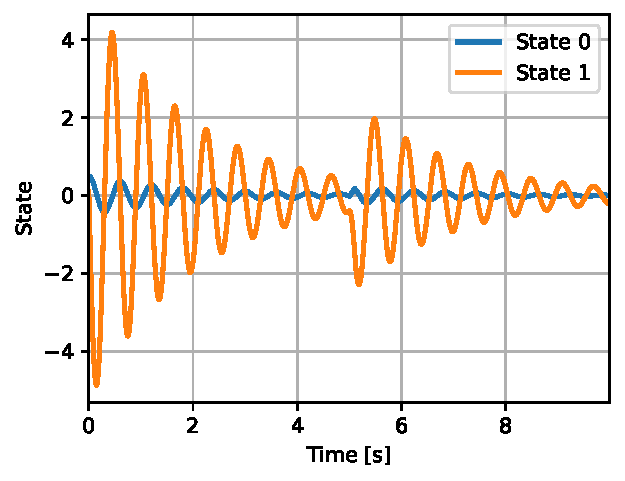
\includegraphics[width=\textwidth]{figures/State_Spring_Damper_(x0_=_[0dot5,_0dot1]).pdf}
    }
    \caption{State of pendulum with spring and damper}
    \label{fig:state-pendulum-spring-damper}
  \end{subfigure}
  \begin{subfigure}[b]{0.49\textwidth}
    { \centering
      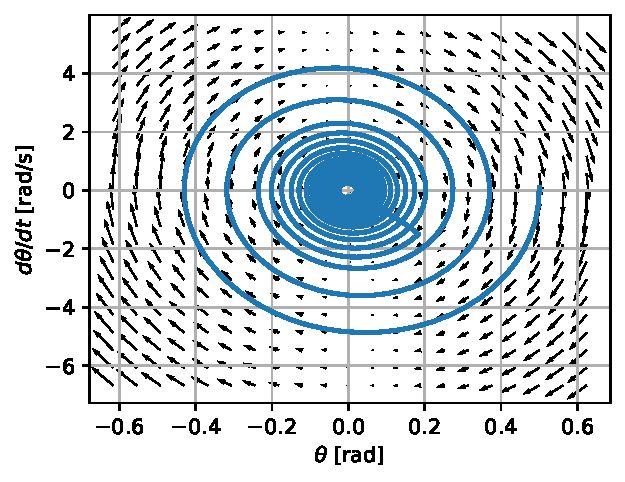
\includegraphics[width=\textwidth]{figures/Phase_Spring_Damper_(x0_=_[0dot5,_0dot1]).pdf}
    }
    \caption{Phase of pendulum with spring and damper}
    \label{fig:phase-pendulum-spring-damper}
  \end{subfigure}
  \caption{\corr{Pendulum setup with spring and damper}}
  \label{fig:pendulum-spring-damper}
\end{figure}

\corr{Note that, like you observed in Lab 2, the nature of the fixed point
  might change depending on the magnitude of the damping term.
  Figure \ref{fig:pendulum-spring-large-damper} shows the behavior
  of the system with the following system parameters,
  \begin{itemize}
  \item $k_1$ = 5.0
  \item $k_2$ = 5.0
  \item $b_1$ = 5.0
  \item $b_2$ = 5.0
  \item $\theta_{ref1} = -45^\circ$
  \item $\theta_{ref2} = 45^\circ$
  \end{itemize}
}
\begin{figure}[H]
  \centering
  \begin{subfigure}[b]{0.49\textwidth}
    { \centering
      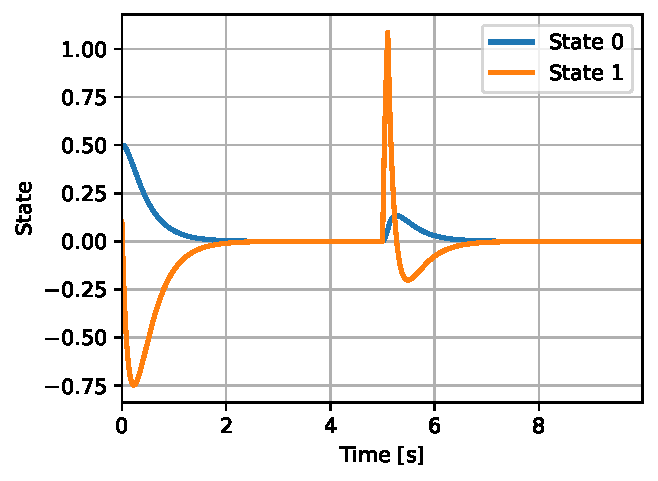
\includegraphics[width=\textwidth]{figures/State_Spring_and_Large_Damping_(x0_=_[0dot5,_0dot1]).pdf}
    }
    \caption{State of pendulum with spring and large damping}
    \label{fig:state-pendulum-spring-large-damper}
  \end{subfigure}
  \begin{subfigure}[b]{0.49\textwidth}
    { \centering
      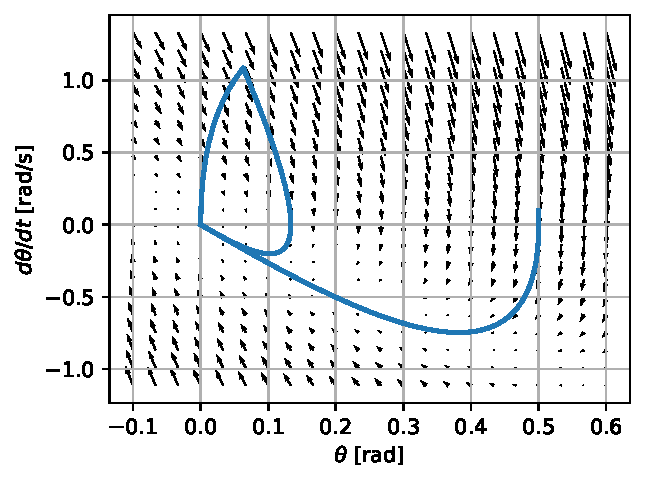
\includegraphics[width=\textwidth]{figures/Phase_Spring_and_Large_Damping_(x0_=_[0dot5,_0dot1]).pdf}
    }
    \caption{Phase of pendulum with spring and large damping}
    \label{fig:phase-pendulum-spring-large-damper}
  \end{subfigure}
  \caption{\corr{Pendulum setup with spring and large damping term. The fixed point now shows an overdamped behavior}}
  \label{fig:pendulum-spring-large-damper}
\end{figure}


\subsection*{2.e Can you find a combination of spring constants ($k$),
  damping constants ($b$) and spring reference angles ($\theta_{ref}$)
  that makes the pendulum rest in a stable equilibrium at
  ($\theta = \pi/6$) radians? Describe how you arrive at the necessary
  parameters and support your response with relevant plots.}


\corr{The following parameters set the pendulum at $\pi/6$
  \begin{eqnarray*}
    b1 = 1. \\
    b2 = 1. \\
    k1 = 50.0 \\
    k2 = 50.0 \\
    s_{theta\_ref1} = np.deg2rad(0.0) \\
    s_{theta\_ref2} = np.deg2rad(65.6)
  \end{eqnarray*}
}

\corr{Using the knowledge from previous questions and setting system
  parameters assymetrically we obtain a pendulum convergence point at
  $\theta = \pi/6$ as shown in figure
  \ref{fig:pendulum-spring-damper-position}.}

\begin{figure}[H]
  \centering
  \begin{subfigure}[b]{0.49\textwidth}
    { \centering
      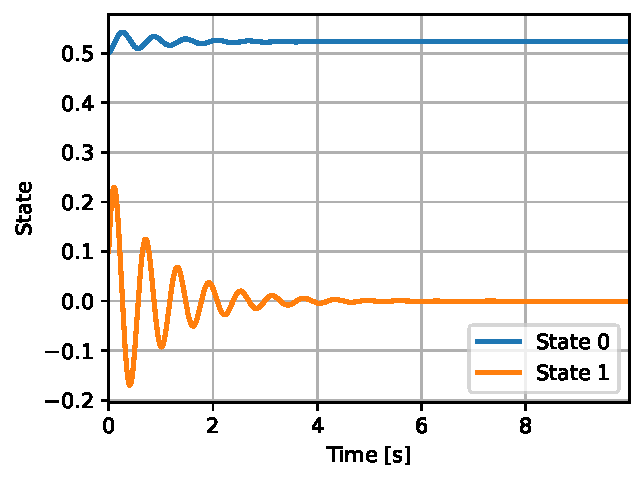
\includegraphics[width=\textwidth]{figures/State_Pendulum_Fixed_Position_(x0_=_[0dot5,_0dot1]).pdf}
    }
    \caption{State of pendulum with spring and damper for a given set
      point}
    \label{fig:state-pendulum-spring-damper-position}
  \end{subfigure}
  \begin{subfigure}[b]{0.49\textwidth}
    { \centering
      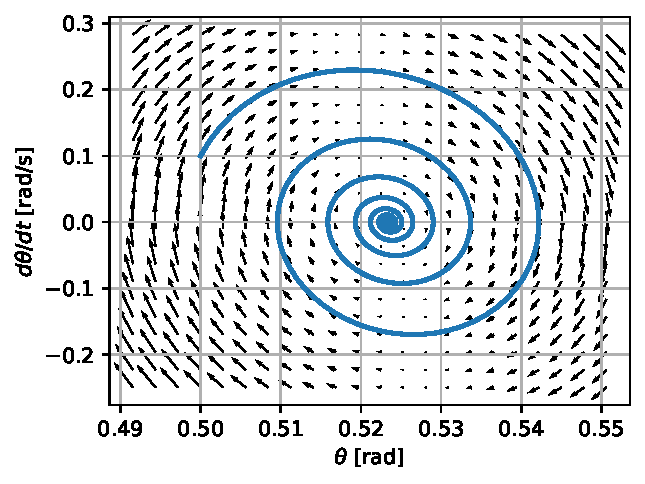
\includegraphics[width=\textwidth]{figures/Phase_Pendulum_Fixed_Position_(x0_=_[0dot5,_0dot1]).pdf}
    }
    \caption{Phase of pendulum with spring and damper for a given set
      point}
    \label{fig:phase-pendulum-spring-damper-position}
  \end{subfigure}
  \caption{\corr{Pendulum setup with spring and damper for a given set
      point}}
  \label{fig:pendulum-spring-damper-position}
\end{figure}

\corr{Note that changing the damping term will not influence the position of the equilibrium point of the system.
  Consider the following parameters:
  \begin{eqnarray*}
    b1 = 1. \\
    b2 = 1. \\
    k1 = 50.0 \\
    k2 = 50.0 \\
    s_{theta\_ref1} = np.deg2rad(0.0) \\
    s_{theta\_ref2} = np.deg2rad(65.6)
  \end{eqnarray*}
  The system still approaches the convergence point in $\theta = \pi/6$, this time
  without damped oscillations, as shown in figure\ref{fig:pendulum-spring-large-damper-position}.
  }

\begin{figure}[H]
  \centering
  \begin{subfigure}[b]{0.49\textwidth}
    { \centering
      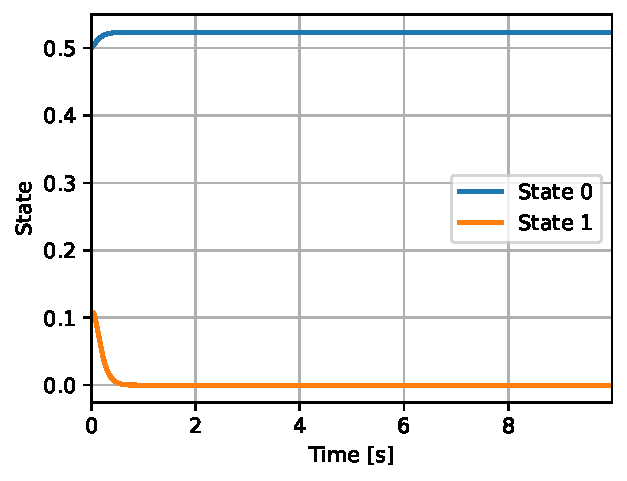
\includegraphics[width=\textwidth]{figures/State_Pendulum_Fixed_Position_with_large_damping_(x0_=_[0dot5,_0dot1]).pdf}
    }
    \caption{State of pendulum with spring and large damping for a given set
      point}
    \label{fig:state-pendulum-spring-large-damper-position}
  \end{subfigure}
  \begin{subfigure}[b]{0.49\textwidth}
    { \centering
      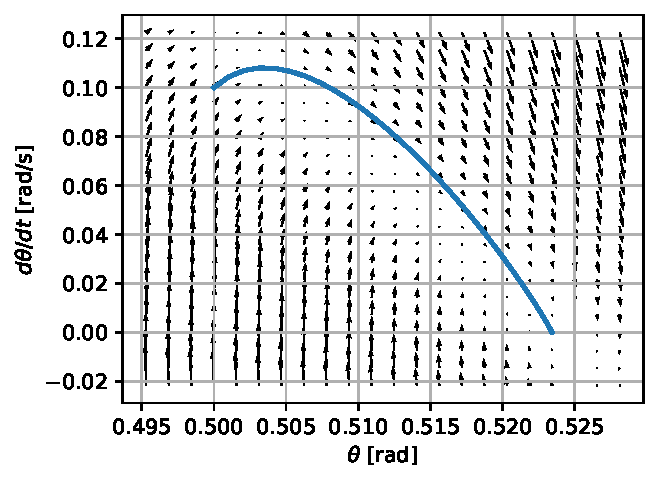
\includegraphics[width=\textwidth]{figures/Phase_Pendulum_Fixed_Position_with_large_damping_(x0_=_[0dot5,_0dot1]).pdf}
    }
    \caption{Phase of pendulum with spring and large damping for a given set
      point}
    \label{fig:phase-pendulum-spring-large-damper-position}
  \end{subfigure}
  \caption{\corr{Pendulum setup with spring and large damping term for a given set
      point}}
  \label{fig:pendulum-spring-large-damper-position}
\end{figure}


\subsection*{2.f What is the missing component between a real muscle
  and the muscle model with passive components that you just explored?
  What behavior's do you lack because of this missing component?}


\corr{The missing component between a real muscle the muscle model
  with passive components is the active contractile element. The
  active contractile element can contract and produce force upon
  receiving an external activation. Having an active element allows
  for an external control to switch the behavior of the pendulum from
  a fixed point behavior to oscillatory and even stable limit cycle
  behaviors}


\end{document}